\chapter{Assumptions About the Distribution of Labels}
\chaptermark{Label Assumptions}
\label{chap:label-assumptions}

\begin{aboutchapter}
In this chapter, we introduce three possible assumptions about the distribution
of node labels and show that none of them is likely to be valid for the
whole database.
To address this problem, we propose two data structures to decide which
assumption to use for a particular set of labels.
\end{aboutchapter}

% \section{Using node labels and relationship types for the estimation of logical
%          result properties}
% \label{sec:node-labels-for-estimation}
%
% As pointed out, node labels are a way for the user to assign a meaning to
% particular groups of nodes. Two nodes having the same label are part of the
% same semantic population defined by the user. It can therefore be assumed that,
% nodes having a particular label tend to share some properties.
%
% With this observation in mind, it seems sensible to base the estimation of
% logical result properties on information corresponding to sets of nodes having
% particular labels.
%
% Additionally, as mentioned before, it can be assumed that the user tends to
% formulate queries which select exactly all nodes having one or several labels.
% Storing helpful information corresponding to these labels allows to estimate
% the logical result properties for such queries very precisely.
%
% Similar arguments can be made in favor of using information corresponding to
% particular relationship types. However, because relationships are defined as
% ordered pairs of nodes, they have to be understood as additional information on
% the nodes in the graph and not as an individual concept.
% It can therefore be argued that, information on relationship types is most
% valuable in conjunction with information on the nodes being connected 
% by the corresponding relationships, i.e. with information on the node labels of
% the connected nodes.
% This argument explains the wide-spread usage of triple statistics
% $(l_1, t, l_2)$ storing the number of relationships of type $t$ starting at
% nodes with label $l_1$ and ending at nodes with label $l_2$, for all labels
% $l_1, l_2$ and relationship types $t$.
%
% To summarize, we will use information corresponding to particular labels and
% relationship types in our estimations.

\section{The Problem of Global Assumptions}
\sectionmark{Global Assumptions}

In the relational algebra, a result of tuples can be filtered according to a
predicate $p$ using the selection operator $\sigma_p$.
Estimating the result cardinality of the selection is equivalent to estimating
the probability of the predicate.

To estimate the probability of a predicate that references multiple attributes,
it is essential to know how the value combinations of these attributes are distributed.
A simple approach is to assume probabilistic independence of the attributes.
The probability of a combination of attribute values is then simply the product
of the individual value probabilities, which are stored in the system catalog.

However, the attribute value independence assumption is often violated in real
data sets (e.g. when there are functional dependencies).
Consequently, research has been done to find better ways of estimating the result
cardinality of multi-attribute selections \cite{poosala_selectivity_1997}.

In our graph algebra, nodes can be filtered using the \op{NodeLabelSelection}
operator.
Suppose the graph DBMS maintains a relation $R$ with schema
$<n, l_1, \ldots, l_i>$, where $n$ is a node and $l_1, \ldots, l_i$ are
Booleans assigning a set of labels to this node.
Estimating the result cardinality of several consecutive label
selections is then equivalent to estimating the result cardinality of a multi-
attribute selection on the $l_1, \ldots, l_i$ attributes of this table.
Consequently, label selections in a graph database can be viewed as a special
case of multi-attribute selections in a relational database.

Take for instance two labels called "Person" and "Student".
Semantically, every student is a person. Therefore
$\selection{v:\text{Student}}(\selection{v:\text{Person}}(\getnodes{v}))
  = \selection{v:\text{Student}}(\getnodes{v})$.
We say that "Student" is a sublabel of "Person" (see Definition
\ref{def:sublabel}).
Obviously, if the database knows about this sublabel relationship, it will make
a far better estimation of the result cardinality than if it assumes e.g.,
independence of students and persons.

\begin{remark}
Relationship types resemble node labels, because they
are also a way of assigning a group membership to a set of entities,
namely relationships.
However, every relationship is exactly of one type. As a result, there is no
uncertainty about the distribution of relationship types, they are disjoint
(unlike node labels).
\end{remark}

Nevertheless, the popular graph database Neo4j always assumes independence
of labels.
In this thesis, we want to demonstrate that cardinality estimates can be
significantly improved by incorporating more information about the node label
distribution. In particular, we consider the cases that labels are
\emph{disjoint} or
in a \emph{sublabel} relation.

\begin{definition}[Sublabels]
\label{def:sublabel}
A label $l'$ is a sublabel of $l$, iff
$\selection{v:l'}(\getnodes{v}) \subseteq \selection{v:l}(\getnodes{v})$.
Equivalently, we call $l$ a superlabel of $l'$.
We denote this relation by $l' \subseteq l$.
\end{definition}

Let us now formalize possible assumptions on the node label distribution.

Take a query result $\Omega$. $\Omega$ can be interpreted as a finite
probability space, such that each subgraph $\mu \in \Omega$ is an elementary
event with probability $\prob{\Omega}(\{\mu\}) = \frac{1}{\card{\Omega}}$.
Then a label selection $\selection{v:l}(\Omega)$ is an event in $\Omega$. We
set $v{:}l := \selection{v:l}(\Omega)$ for readability. The probability of
drawing a subgraph from $\Omega$ where the node matched by the variable $v$
has label $l$ is given as
\begin{align}
  \prob{\Omega}(v{:}l) = \frac{\card{\selection{v:l}(\Omega)}}{\card{\Omega}}
  \label{eq:label-probability}
\end{align}

The problem is to estimate the probability
\[
  \prob{\Omega} \lb \bigisect_{l \in L} v{:}l \rb
\]
for a set $L \subseteq \nlabels$ of node labels.
We write $v{:}L$ as a short-hand for $\bigisect_{l \in L} v{:}l$.

We already suggested that, making a global assumption about
the relationship of all pairs of labels $l_1, l_2 \in L$ is error-prone.
To illustrate this fact, we look at three different
global assumptions and the corresponding estimation formulas.
\begin{enumerate}
  \item Suppose the labels form a subset chain, i.e., for all $l_1, l_2 \in L$
    it holds either $l_1 \subseteq l_2$ or $l_2 \subseteq l_1$.
    Then
    \[
      \prob{\Omega}(v{:}L) = \min_{l \in L} \prob{\Omega}(v{:}l)
      \label{ass:chain}
    \]
  \item Suppose the labels are pair-wise independent, i.e., for all $l_1, l_2 \in L$
    it holds that
    $\prob{\Omega}(v{:}l_1 \isect v{:}l_2) = \prob{\Omega}(v{:}l_1) \cdot \prob{\Omega}(v{:}l_2)$.
    Then
    \[
      \prob{\Omega}(v{:}L) = \prod_{l \in L} \prob{\Omega}(v{:}l)
      \label{ass:ind}
    \]
  \item Suppose there are two labels $l_1, l_2 \in L$ that are disjoint, i.e.,
    $\prob{\Omega}(v{:}l_1 \isect v{:}l_2) = 0$.
    Then
    \[
      \prob{\Omega}(v{:}L) = 0
      \label{ass:disj}
    \]
\end{enumerate}

Without any knowledge about the database graph, it is
impossible to tell which of these assumptions should be preferred.
In particular, we have no reason to choose the independence assumption, other
than assuming that our database will only be used for datasets where node
labels are independent.

Moreover, none of these assumptions is likely to be valid for
all subsets of labels $L$.
From a user perspective, it seems very probable that there will be labels
that are in a sublabel relation (recall the example on students and persons
above) and at the same time labels that are disjoint (consider for instance
two labels "Male" and "Female").
Hence, we need means to decide which assumption to use for a given set of labels.

\begin{remark}
Note that labels being disjoint or in a sublabel relation does not imply
that there is a functional dependency between the attributes representing
these labels in the relation $R$ described above:

If two labels $l_1, l_2$ are disjoint, there are no nodes having both of
these labels, i.e., there are no tuples $t \in R$
with $t[l_1] = \true = t[l_2]$.
% However, it is possible that two tuples $t_1, t_2 \in R$ with
% $t_1[l_1] = \false$, $t_1[l_2] = \false$, $t_2[l_1] = \false$ and
% $t_2[l_2] = \true$.
Similarly, if $l_1 \subseteq l_2$, there are no nodes having $l_1$ but not
$l_2$, i.e., there are no tuples $t \in R$ with $t[l_1] = \true$ and
$t[l_2] = \false$.
However, in both cases it is possible that two tuples $t_1, t_2 \in R$ with
$t_1[l_1] = \false$, $t_1[l_2] = \false$, $t_2[l_1] = \false$ and
$t_2[l_2] = \true$.

Consequently, techniques for functional dependency discovery are not suitable
for the discovery of sublabels or disjoint labels.
\end{remark}

\section{Storing More Information}
\label{sec:more-label-info}

We will now introduce two data structures that allow us to decide
which assumption to use for a given set of labels.

\subsection{Label Partition}
\label{sub:label-partition}

First of all, we divide the set of labels $\nlabels$ in the database graph
into subsets of \emph{overlapping} labels, that form a partition $\lpart$ of
this set. For a given label $l$, we denote the member set of $\lpart$
containing $l$ as $\lpart(l)$.
If two labels are in different member sets of $\lpart$, we will assume they
are disjoint.
We refer to such a partition as a \emph{label partition}.

A label partition may be provided \emph{a priori} by the user.
It can then be understood as a contract:
The user does not intend to assign two labels from different member
sets of the partition to the same node.

A label partition can also be built \emph{a posteriori} by the DBMS, e.g.
using a clustering algorithm.
The distance measure for two labels $l_1, l_2$ is the
Jaccard distance between their sets of nodes:
\begin{align}
\begin{split}
  \label{eq:jacc-dist}
  d(l_1, l_2) &= \jaccdist(\selection{v:l_1}(\getnodes{v}),
                           \selection{v:l_2}(\getnodes{v})) \\
              &= 1 - \frac{\card{\selection{v:l_1}(
                                 \selection{v:l_2}(\getnodes{v}))}}
                          {\card{\selection{v:l_1}(\getnodes{v}) \union
                                 \selection{v:l_2}(\getnodes{v})}}
\end{split}
\end{align}
The clusters produced by an algorithm using this distance measure represent the
wanted partition. Obviously, the result strongly depends on the chosen
algorithm and its parameters.

To better understand the intention of the label partition, consider the following
example. Suppose we have a database about movies. Figure \ref{fig:label-dist-example}
shows the distribution of the different labels among the nodes of this database as a
Venn diagram.

\begin{figure}[h]
  \centering
  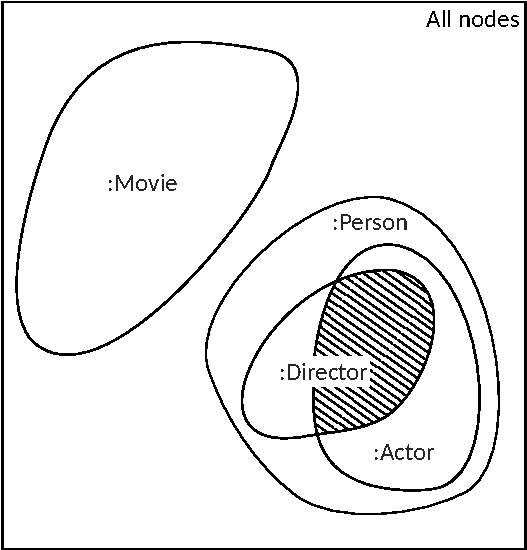
\includegraphics[width=0.4\textwidth]{figures/nodes-venn-diagram.pdf}
  \caption{Distribution of node labels in a example database.}
  \label{fig:label-dist-example}
\end{figure}

From this diagram, we can conclude that movies and persons are disjoint.
We also see that, persons, actors and directors do strongly overlap.
Consequently, the following label partition might be a good choice:
\[
  \lpart := \{ \{ \text{Movie} \},
               \{ \text{Person}, \text{Actor}, \text{Director} \} \}
\]

We highlight one option for a partition, which we call the
\emph{strict partition}. First, we define a relation for overlapping labels:
\begin{align}
\begin{split}
  &\overlap \subseteq \nlabels^2 \\
  &l_1 ~\overlap~ l_2 ~:\Leftrightarrow~
    \selection{v:l_1}(\selection{v:l_2}(\getnodes{v})) \not = \emptyset
\end{split}
\end{align}
$\overlap$ is reflexive and symmetric and the transitive closure
$\overlap^+$ is thus an equivalence relation.

The strict partition $\strictlpart$ is simply the set of equivalence classes
of $\overlap^+$ (also called the quotient set):
\begin{align}
\begin{split}
  \strictlpart &:= \nlabels / \overlap^+ \\
               &= \{ \{ l' \in \nlabels \mid l ~\overlap^+~ l' \}
                      \mid l \in \nlabels \}
\end{split}
\end{align}

We observe that labels from different equivalence classes are disjoint:
Take two labels $l_1, l_2$ from different equivalence classes
$O_1, O_2 \in \strictlpart$. Then $(l_1, l_2) \not \in \overlap^+$.
This implies $(l_1, l_2) \not \in \overlap$ and therefore
$\selection{v:l_1}(\selection{v:l_2}(\getnodes{v})) = \emptyset$.
Note that the inverse is not necessarily true, there may be two labels in the
same equivalence class which are disjoint (this is a potential weakness of the
strict partition, see the remark below).

As a result, if $L \subseteq \nlabels$ contains two labels from different
members of $\strictlpart$ then $\prob{\Omega}(v{:}L) = 0$ for any query result
$\Omega$.

\begin{remark}
The strict partition can also be obtained using a single-linkage
hierarchical clustering that succesively merges all clusters of labels
having a cluster distance smaller than $1$ (using the Jaccard distance
measure defined in Equation \ref{eq:jacc-dist}).
Once the single-linkage algorithm has finished, two
labels from different clusters will have distance $1$, which means that their
node sets are disjoint.

Because the single-linkage algorithm tends to build long chains, it can happen
that many pairs of disjoint node labels end up in the same cluster.
This can be avoided by a different linkage criterion (e.g. average linkage).
\end{remark}

\subsection{Sublabel Map}
\label{sub:sublabel-map}

In addition to the partition, we generate a \emph{sublabel map} $\submap$.
The sublabel map assigns to each label all labels that are considered to be
sublabels of this label. Again, this map can be provided by the user or 
maintained by the DBMS.

In the example of Figure \ref{fig:label-dist-example}, a good sublabel map
would be
\begin{align*}
  &\submap(\text{Movie}) := \emptyset \\
  &\submap(\text{Person}) := \{ \text{Actor}, \text{Director} \} \\
  &\submap(\text{Actor}) := \emptyset \\
  &\submap(\text{Director}) := \emptyset
\end{align*}

We define the \emph{strict sublabel map} as
\begin{align}
\begin{split}
  &\strictsubmap ~:~ \nlabels \rightarrow \powSet{\nlabels} \\
  &\strictsubmap(l) :=  \{ l' \in \nlabels \mid l' \subseteq l \}
\end{split}
\end{align}
Following this definition, if $l' \in \strictsubmap(l)$, then it follows
logically for all query results $\Omega$ that
$\prob{\Omega}(v{:}l \isect v{:}l') = \prob{\Omega}(v{:}l')$.

\begin{remark}
Again, the condition for the assumption of a sublabel relationship can be
weakened if necessary.
A straightforward option is the following definition of the sublabel map
\[
  \submap(l) :=  \{ l' \in \nlabels \mid
    \frac{\card{\selection{v:l'}(\selection{v:l}(\getnodes{v}))}}
         {\card{\selection{v:l'}(\getnodes{v})}} \geq \epsilon \}
\]
which considers those labels $l'$ sublabels of $l$ whose nodes are contained in
the nodes of $l$ to a (tunable) degree $\epsilon$.
\end{remark}

\section{Solving the Problem of Global Assumptions}
\sectionmark{Solution}

We will now show how to address the problem of global assumptions using a label
partition $\lpart$ and a sublabel map $\submap$.

Suppose a set $L \subseteq \nlabels$ of node labels.

If there are two node labels $l_1, l_2 \in L$ with
$\lpart(l_1) \not = \lpart(l_2)$, then the label partition tells us we should
assume $\prob{\getnodes{v}}(v{:}l_1 \isect v{:}l_2) = 0$. This implies
$\prob{\Omega}(v{:}l_1 \isect v{:}l_2) = 0$ and therefore
\[
  \prob{\Omega}(v{:}L) \approx 0 ~\text{.}
\]

On the contrary, if all labels from $L$ are in the same member set of $\lpart$,
we make use of the sublabel map to simplify the probability expression.
Take a label $l \in L$. If $s(l) \isect L \not = \emptyset$ then the sublabel
map tells us to assume that $L$ contains a sublabel $l' \subseteq l$.
This means that
$\prob{\getnodes{v}}(v{:}l' \isect v{:}l) \approx \prob{\getnodes{v}}(v{:}l')$
and implies
$\prob{\Omega}(v{:}l' \isect v{:}l) \approx \prob{\Omega}(v{:}l')$.

Iterative application of this simplification gives us a smaller set of labels
$L' := \{ l \in L \mid s(l) \isect L = \emptyset \}$, with
\[
  \prob{\Omega}(v{:}L) \approx \prob{\Omega}(v{:}L') ~\text{.}
\]

Now we are left with a set of labels $L'$, which contains overlapping labels
that are not sublabels of each other.
We do now finally assume these labels are independent in $\Omega$, which
gives us the solution
\[
  \prob{\Omega}(v{:}L) \approx \prod_{l \in L \land s(l) \isect L = \emptyset}
                                 \prob{\Omega}(v{:}l)
\]

All in all, we can compute the probability of drawing a subgraph where the
nodes matched by $v$ have the labels $L$ as
\begin{align}
  \prob{\Omega}(v{:}L) \approx
                         \begin{cases}
                           0, \text{ if there are } l_1, l_2 \in L
                              \text{ such that } D(l_1) \not = D(l_2) \\
                           \prod_{l \in L \land s(l) \isect L = \emptyset}
                             \prob{\Omega}(v{:}l), \text{ otherwise}
                         \end{cases}
\end{align}

For instance, in the example of Figure \ref{fig:label-dist-example}, using the
proposed label partition and sublabel map, we have
\begin{align*}
  \prob{\Omega}(v{:}\text{Person} \isect v{:}\text{Actor}
                \isect v{:}\text{Director})
    &\approx \prob{\Omega}(v{:}\text{Actor})
             \cdot \prob{\Omega}(v{:}\text{Director})
\end{align*}
\[
  \prob{\Omega}(v{:}\text{Director} \isect v{:}\text{Movie}) \approx 0
\]
